\documentclass[11pt,a4paper]{article}
\usepackage[utf8]{inputenc}
\usepackage[spanish]{babel}	%Idioma
\usepackage{amsmath}
\usepackage{url}
\makeatletter
\g@addto@macro{\UrlBreaks}{\UrlOrds}
\makeatother
\usepackage{amsfonts}
\usepackage{amssymb}
\usepackage{graphicx} 	%Añadir imágenes
\usepackage{geometry}	%Ajustar márgenes
\usepackage[export]{adjustbox}[2011/08/13]
\usepackage{float}
\restylefloat{table}
\usepackage[hidelinks]{hyperref}
\usepackage{titling}
\graphicspath{}
%\usepackage{minted}
\usepackage{multirow}
\usepackage{caption}
\usepackage{multicol}
\usepackage{array}
\usepackage[hyphenbreaks]{breakurl}
\usepackage[hyphens]{url}
\PassOptionsToPackage{hyphens}{url}\usepackage{hyperref}
\usepackage{eurosym}


%Opciones de encabezado y pie de página:
\usepackage{fancyhdr}
\pagestyle{fancy}
\lhead{Grado en Ingeniería Informática}
\rhead{Man In The Middle}
\lfoot{Servidores Web de Altas Prestaciones}
\cfoot{}
\rfoot{\thepage}
\renewcommand{\headrulewidth}{0.4pt}
\renewcommand{\footrulewidth}{0.4pt}

%Opciones de fuente:
\usepackage[utf8]{inputenc}
\usepackage[default]{sourcesanspro}
\usepackage{sourcecodepro}
\usepackage[T1]{fontenc}

\setlength{\parindent}{15pt}
\setlength{\headheight}{15pt}
\setlength{\voffset}{10mm}

% Custom colors
\usepackage{color}
\definecolor{deepblue}{rgb}{0,0,0.5}
\definecolor{deepred}{rgb}{0.6,0,0}
\definecolor{deepgreen}{rgb}{0,0.5,0}
\hypersetup{
    colorlinks=true,
    linkcolor=black,
    urlcolor=blue,
}

\usepackage{listings}

\begin{document}
\sloppy
\begin{titlepage}

\begin{minipage}{\textwidth}

\centering
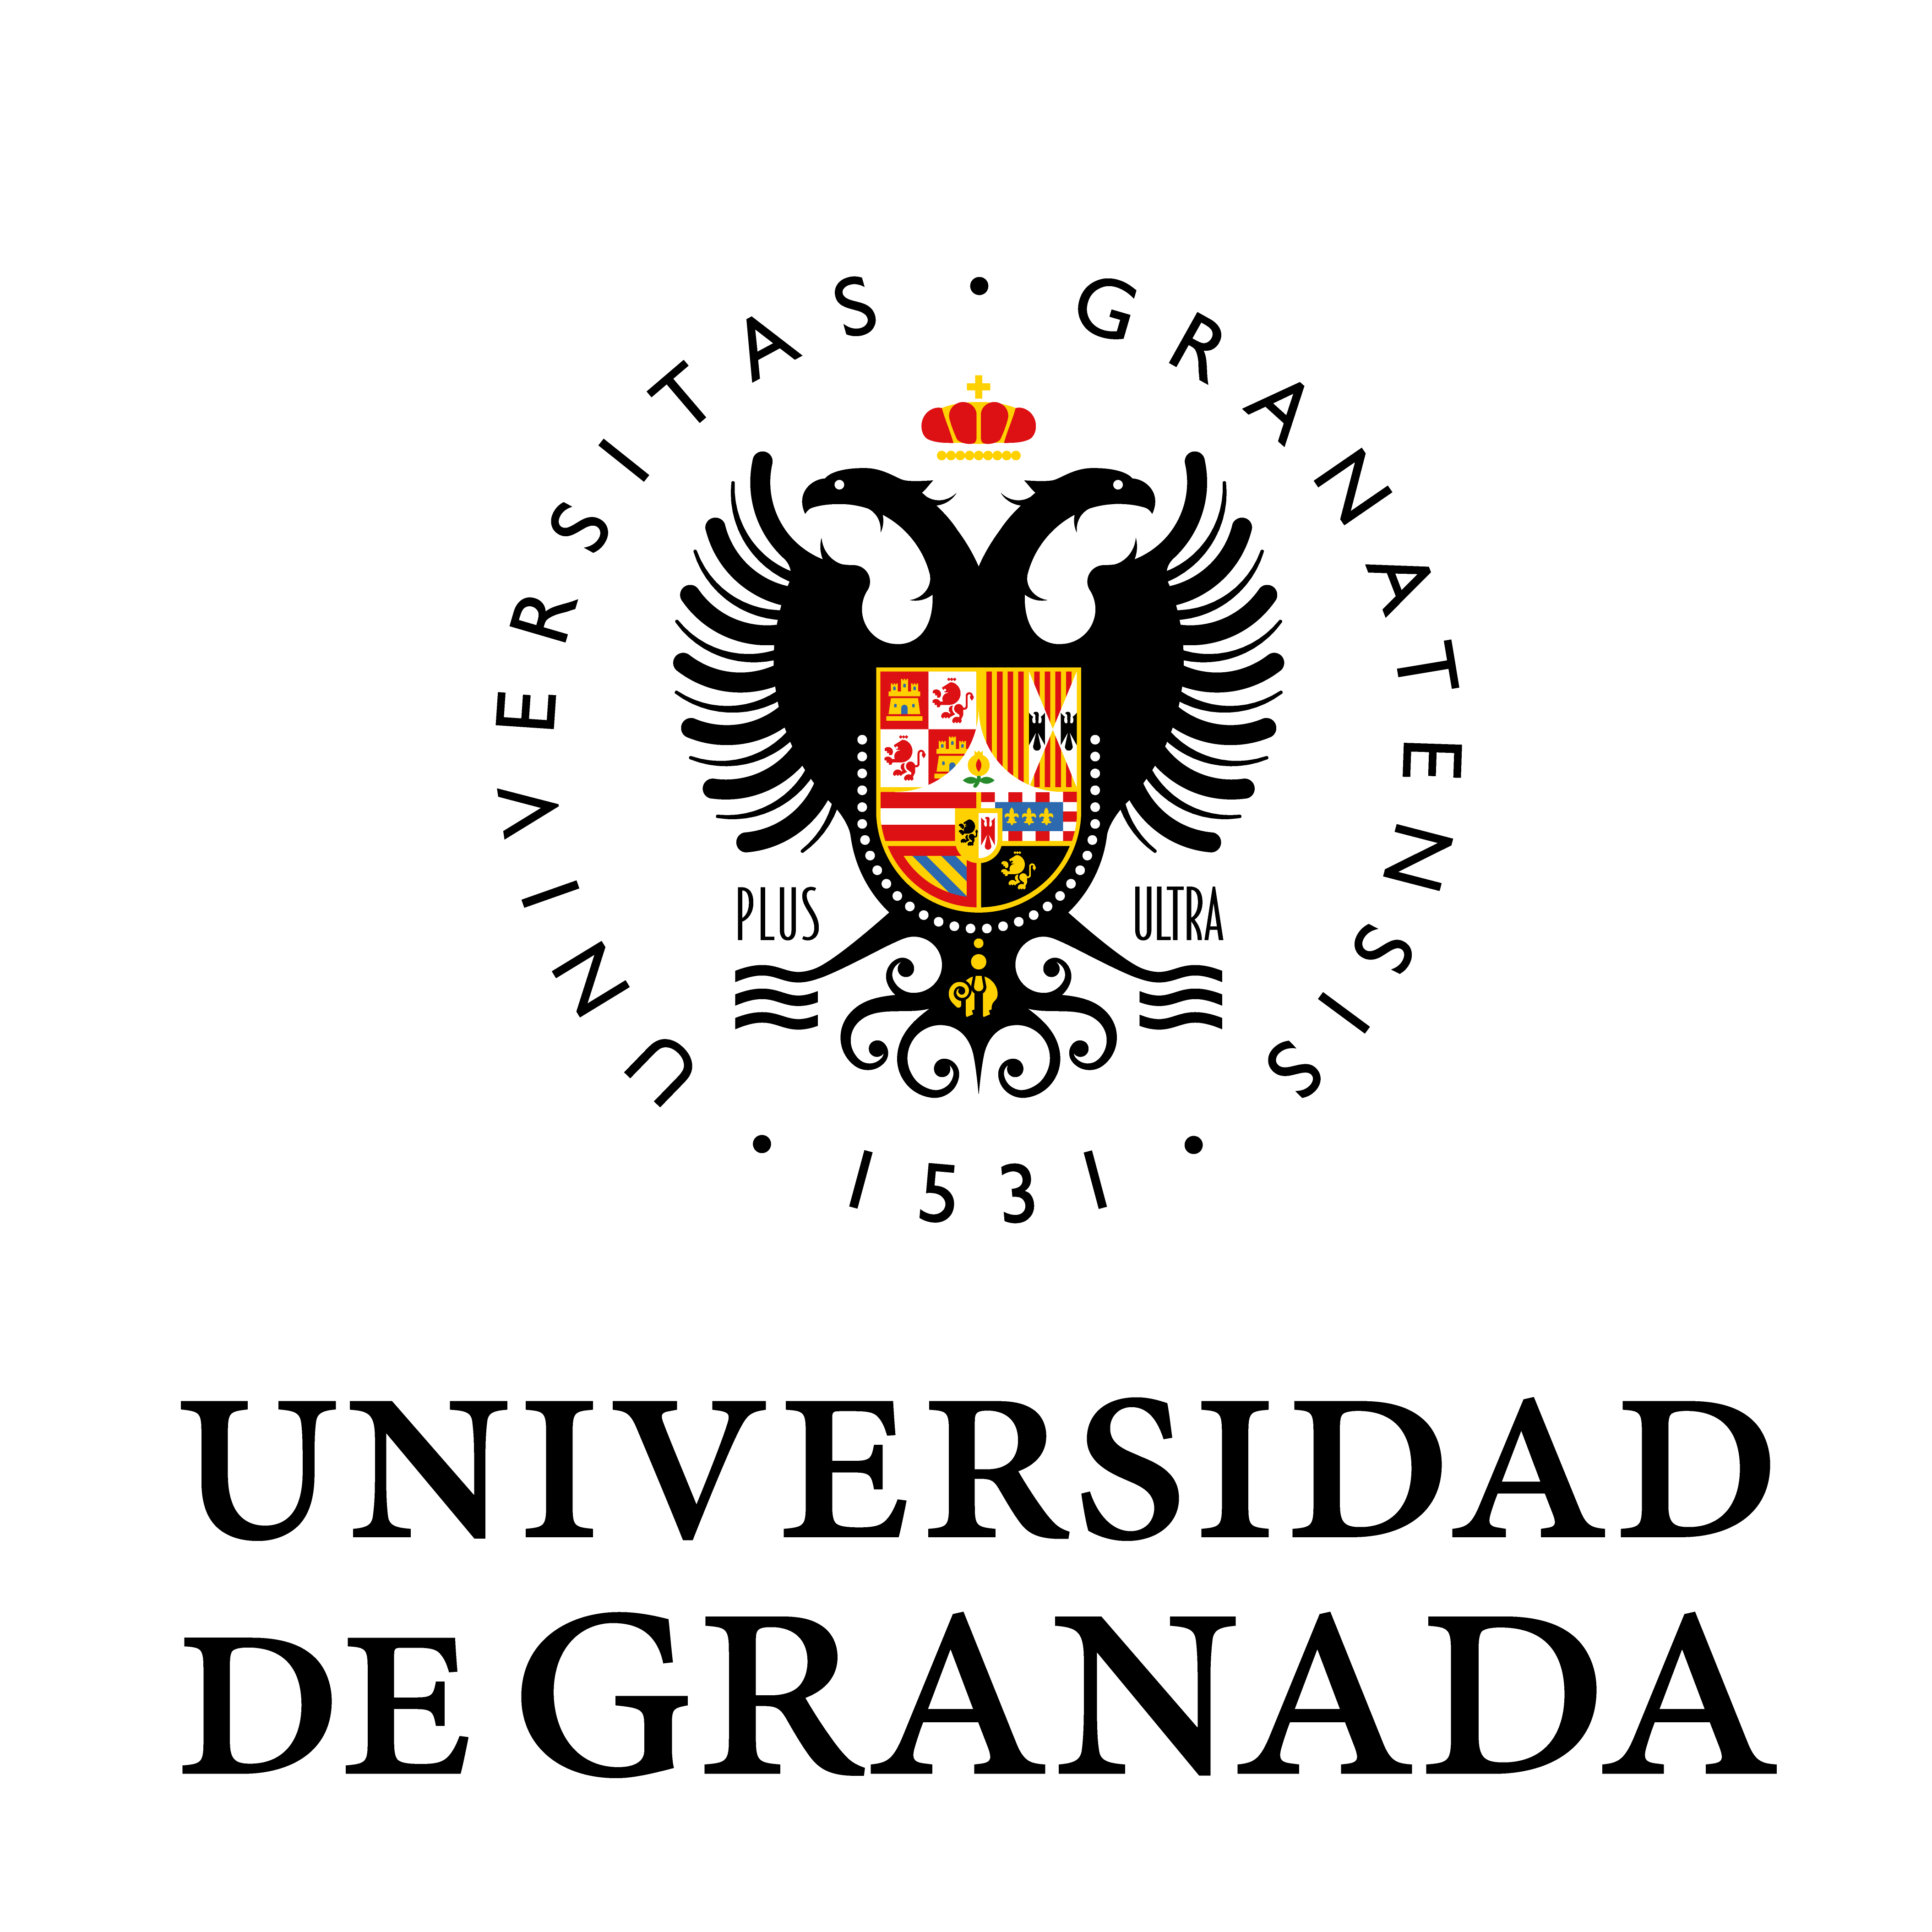
\includegraphics[width=0.5\textwidth]{logo.png}\\

\textsc{\Large Servidores Web de Altas Prestaciones\\[0.2cm]}
\textsc{GRADO EN INGENIERÍA INFORMÁTICA}\\[1cm]

{\Huge\bfseries Ataques Man-In-The-Middle\\}
\noindent\rule[-1ex]{\textwidth}{3pt}\\[3.5ex]
{\large\bfseries}
\end{minipage}

\vspace{1.5cm}
\begin{minipage}{\textwidth}
\centering

\textbf{Autores}\\ {Elena María Gómez Ríos\\Nazaret Román Guerrero\\Guillermo Sandoval Schmidt}\\[2.5ex]

\includegraphics[width=0.3\textwidth]{etsiit.jpeg}\\[0.1cm]
\vspace{1cm}
\textsc{Escuela Técnica Superior de Ingenierías Informática y de Telecomunicación}\\
\vspace{1cm}
\textsc{Curso 2018-2019}
\end{minipage}
\end{titlepage}

\pagenumbering{gobble}
\pagenumbering{arabic}
\tableofcontents
\thispagestyle{empty}

\newpage

\section{¿Qué es?}

Un ataque \textbf{\textit{Man-In-The-Middle}} es un ataque en el que se consigue la capacidad de leer, modificar y reenviar datos a voluntad. De esta forma se puede acceder al contenido privado como, por ejemplo, datos confidenciales y contraseñas.\\

La sutileza del ataque se basa en que todo tiene que suceder sin que el cliente y el servidor o el cliente y el cliente entre los que se realiza la conexión se den cuenta de que hay un infiltrado entre ellos. Este tipo de ataques criptográficos tienen especial interés cuando se lleva a cabo el intercambio de \textit{Diffie-Hellman} sin autenticación.

\section{Software para realizar un ataque MITM}

Hemos utilizado una máquina virtual con Kali Linux para realizar el ataque ya que tiene instaladas las aplicaciones necesarias para este tipo de ataques, como por ejemplo Ettercap, que es la aplicación que nosotros hemos utilizado.\\

Actualmente existen una gran cantidad de programas para realizar ataques \textit{Man-In-The-Middle}. Por ejemplo, se podría utilizar WireShark que es un potente sniffer de red con el que se pueden ver posibles ataques. Otro programa es mitmAP que está escrito en python e incorpora otras herramientas para realizar este tipo de ataque. Otros ejemplos son: Bettercap, MITMProxy, Evilgrade, Hamster o Ferret.

\section{¿Cómo defenderse ante un ataque MITM?}

A pesar de ser un ataque básico y ser conocido por todos en el ámbito, sigue siendo uno de los principales ataques de seguridad que se pueden llevar a cabo. Para poder defenderse de este, se pueden utilizar mecanismos como los siguientes:

\begin{itemize}
    \item \textbf{Claves públicas.} En este caso, se cifran los mensajes con la clave privada del primer sujeto y el sujeto B lo descifra con la clave pública. De esta forma, el sujeto intermedio no conoce la clave pública que comparten ni tampoco tiene una clave privada que descifre el mensaje, de forma que la conexión es asimétrica y segura.
    \item \textbf{Claves secretas (con alta entropía).} Similar al caso anterior pero teniendo en cuenta la entropía de las claves, es decir, la información que muestran los símbolos que forman la llave. En el caso de, por ejemplo, una clave de texto, las palabras más ``raras'' son las que tienen mayor entropía y las que ofrecen mayor información.
    \item \textbf{Técnicas biométricas.} Difíciles de suplantar para poder actuar como un intermediario de las conexiones, como por ejemplo reconocimiento de voz, escáner de huellas dactilares o de retina...
    \item \textbf{HTTPS.} Asegurarse de que la conexión se realiza a través de un canal seguro para evitar accesos indeseados a los datos.
    \item \textbf{Conexiones VPN.} Conectarse a una red WIFI pública conlleva peligros como una exposición directa a ataques de este tipo. Utilizar una conexión privada es mucho más segura que utilizar una conexión pública asegurada con métodos anteriores.
    \item \textbf{Malware.} A la hora de descargar software, hay que hacerlo de sitios seguros y de confianza, para evitar que el software descargado contenga malware que pueda afectar a nuestras conexiones.
    \item \textbf{Actualizaciones.} Mantener el software utilizado actualizado, ya que, cuanto más antiguo es el software, más fácil es que se hayan encontrado debilidades expongan la seguridad.
\end{itemize}

\section{Ataques famosos}

\begin{itemize}
    \item En 2015, 49 personas fueron detenidas en Europa tras una operación organizada por la Europol. Los hackers, mediante una técnica de ``phising'' se quedaban con datos de los clientes de varios bancos, engañandolos utilizando un página prácticamente idéntica a la original de dichos bancos. De este modo, las transferencias en lugar de llegar al destino intencionado, llegaban a los estafadores, llegando a conseguir de manera fraudulenta cerca de 6.000.000\euro.
    
    \item Sin irnos más lejos, en 2016, en España, una joven de 19 años fue detenida tras realizar un ataque MITM a una empresa, suplantando la identidad de esta y estafando 6.500\euro \hspace de la misma, ya que modificó el número de cuenta original al que iba dirigida la transferencia.
    
    \item Quizás uno de los casos más conocidos de ataque MITM y que fue destapado por Edward Snowden, fue el perpetrado por la Agencia Nacional de Seguridad Estadounidense, que simulaba los servicios de búsqueda de Google para recolectar datos de los usuarios. 
    
\end{itemize}

\section{Actuando como intermediario}

Ahora es nuestro turno de llevar a cabo un ataque. Para ello, y utilizando el software descrito anteriormente, descubriremos el usuario y la contraseña de un cliente que se conectará a una página web sin seguridad.

\subsection{Configuración del cortafuegos de la máquina atacante}

Para configurar el cortafuegos al iniciar la máquina, hemos utilizado un script de bash que ejecute los comandos necesarios para configurar \textit{iptables.} El script es el que sigue:

\begin{lstlisting}[language=bash,caption={bash version},captionpos=b]
#!/bin/bash
iptables -F
iptables -X
iptables -Z
iptables -t nat -F

iptables -P FORWARD ACCEPT
iptables -t nat -A POSTROUTING -o eth0 -j MASQUERADE
iptables -t nat -A PREROUTING -i eth1 -p tcp --destination-port 80 
         -j REDIRECT --to-port 10000

iptables-save > /etc/iptables.up.rules
\end{lstlisting}

Con esto hemos conseguido infiltrarnos en la conexión y enmascarar nuestra presencia, fingiendo que somos el cliente cuando los paquetes provengan del servidor, y el servidor cuando los paquetes provengan del cliente.

\subsection{Situándonos entre las víctimas}

Para este paso es necesario utilizar el software \textit{Ettercap}.

\begin{enumerate}
    \item Comenzamos a esnifar la conexión con \textsc{sniff}$\rightarrow$\textsc{unified sniffing}.
    \item Detectamos los hosts que hay en nuestra red y a los que vamos a atacar.
        \begin{figure}[H]
            \centering
            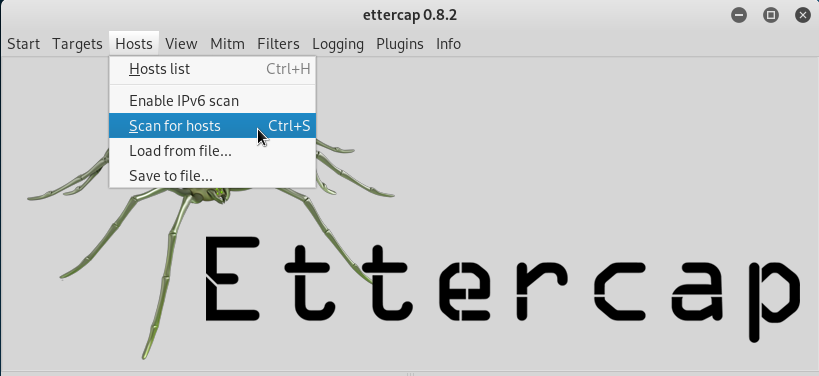
\includegraphics[width=1.0\textwidth]{scan_host.png}\\[0.1cm]
            \caption{Escaneado de hosts}
            \label{fig:my_label}
        \end{figure}
        \begin{figure}[H]
            \centering
            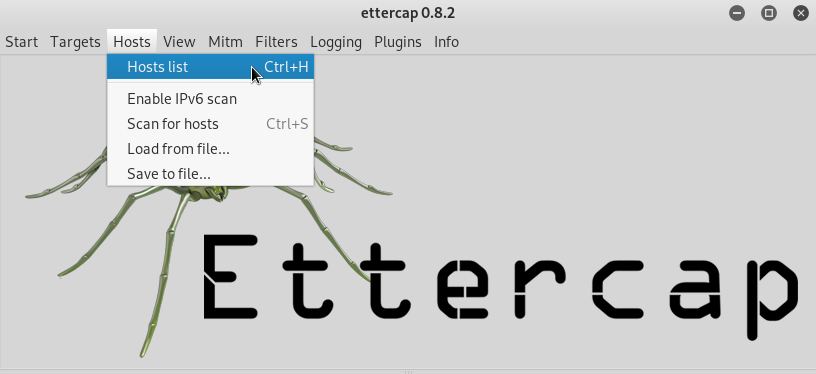
\includegraphics[width=1.0\textwidth]{host_list.png}\\[0.1cm]
            \caption{Lista de máquinas}
            \label{fig:my_label}
        \end{figure}
        \begin{figure}[H]
            \centering
            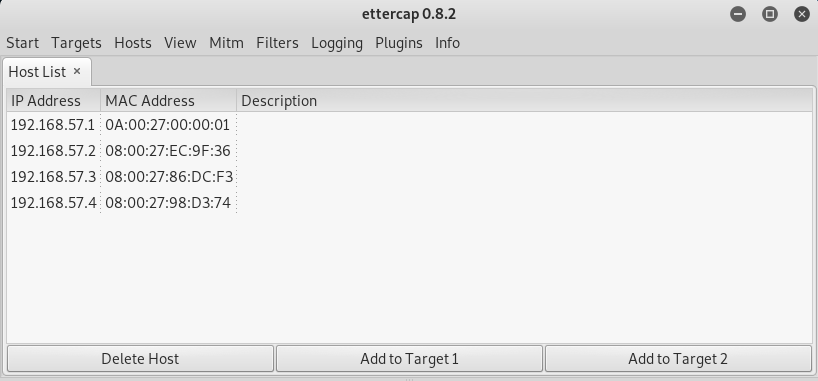
\includegraphics[width=1.0\textwidth]{lista.png}\\[0.1cm]
            \caption{Hosts disponibles}
            \label{fig:my_label}
        \end{figure}
    \item Paramos el sniffing con \textsc{sniff}$\rightarrow$\textsc{stop sniffing}.
    \item Añadimos cada host a un \textsc{target}, seleccionando el host y clickando en \textsc{add to target1}. Nuestros host son el 192.168.57.3 (como servidor) y el 192.168.57.4 (como cliente).
    \item Ahora hay que hacer un envenenamiento del protocolo ARP para que, en la ruta, entremos nosotros como punto intermedio al que pasarle los datos.
        \begin{figure}[H]
            \centering
            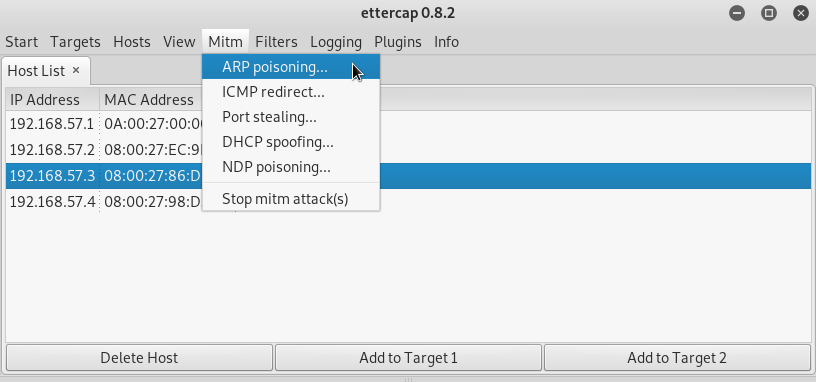
\includegraphics[width=1.0\textwidth]{pois.png}\\[0.1cm]
            \caption{Envenamiento de ARP}
            \label{fig:my_label}
        \end{figure}
    \item Comenzamos con el proceso de sniffing de nuevo con la conexión envenenada.
    \item Accedemos desde el cliente a la página.
    \begin{figure}[H]
        \centering
        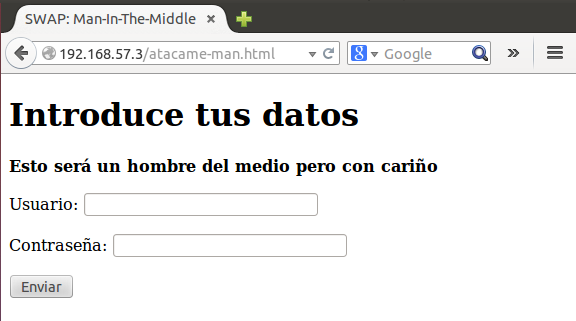
\includegraphics[width=1.0\textwidth]{formulario.png}\\[0.1cm]
        \caption{Formulario}
        \label{fig:my_label}
    \end{figure}
    \item Eliminamos la desencriptación de las peticiones.
        \begin{figure}[H]
            \centering
            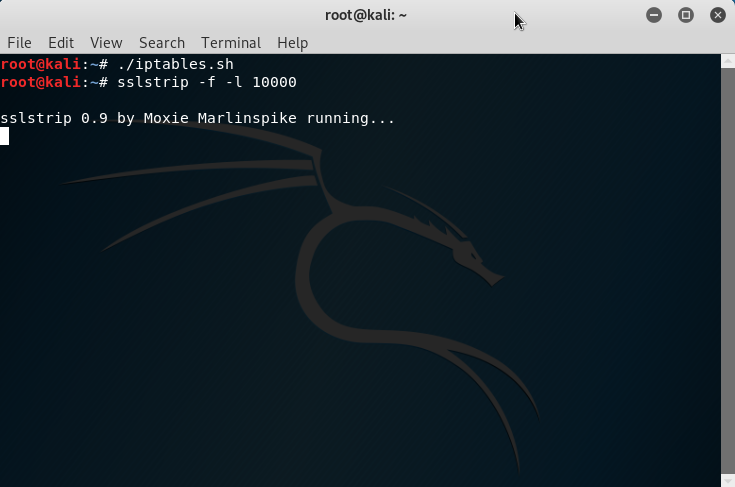
\includegraphics[width=1.0\textwidth]{sslstrip.png}\\[0.1cm]
            \caption{SSLstrip}
            \label{fig:my_label}
        \end{figure}
    \item Finalmente, hemos conseguido el usuario y la contraseña.
        \begin{figure}[H]
            \centering
            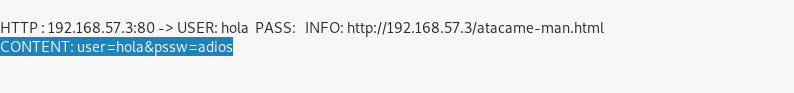
\includegraphics[width=1.0\textwidth]{ataque.png}\\[0.1cm]
            \caption{MITM}
            \label{fig:my_label}
        \end{figure}
\end{enumerate}


\section{Bibliografía}
\begin{itemize}
    \item \url{https://en.wikipedia.org/wiki/Man-in-the-middle_attack}
    \item \url{https://en.wikipedia.org/wiki/Entropy_(information_theory)}
    \item \url{http://www.cursodehackers.com/ManInTheMiddle.html}
    \item \url{https://us.norton.com/internetsecurity-wifi-what-is-a-man-in-the-middle-attack.html}
    \item \url{https://www.cnet.com/news/nsa-disguised-itself-as-google-to-spy-say-reports/}
    \item \url{https://nakedsecurity.sophos.com/es/2015/06/11/49-busted-in-europe-for-man-in-the-middle-bank-attacks/}
    \item \url{https://navarra.elespanol.com/articulo/sucesos/detenida-pamplona-joven-19-anos-estafar-6-500-euros-empresa/20160513113625041253.html}
\end{itemize}

\end{document}